\chapter{Sensor Data}

%Replace \lipsum with text.
% You may have as many sections as you please. This is just for reference.

\section{Sensor Tile Kit}

% TODO: Add android code screenshot that shows the limitation
In section \ref{ch1-intro-android}, we explained how Android limits the sensor data sampling rate to around 200Hz, which is good enough for monitoring device movements, such as tilt, rotation etc.
% TODO: Fix this line
but is low for our goal to use it as an microphone since human audible frequencies lie in the 20Hz to 20kHz range.
To explore what could be done if we had access to high frequency sensor data, we tried a specialized sensor board - the SensorTile by STMicroelectronics.

The SensorTile is a tiny, square-shaped IoT module that packs powerful processing capabilities leveraging an 80 MHz microcontroller, a Bluetooth low energy connectivity based on BlueNRG-MS network processor as well as a wide spectrum of motion, such as a triaxial accelerometer, gyroscope, magnetometer, and environmental sensors, such as pressure, humidity and temperature and even a digital microphone. \cite{stkit}

Figure \ref{fig:sensortilekit} shows the contents of the SensorTile kit.

\begin{figure}[H] \begin{center}
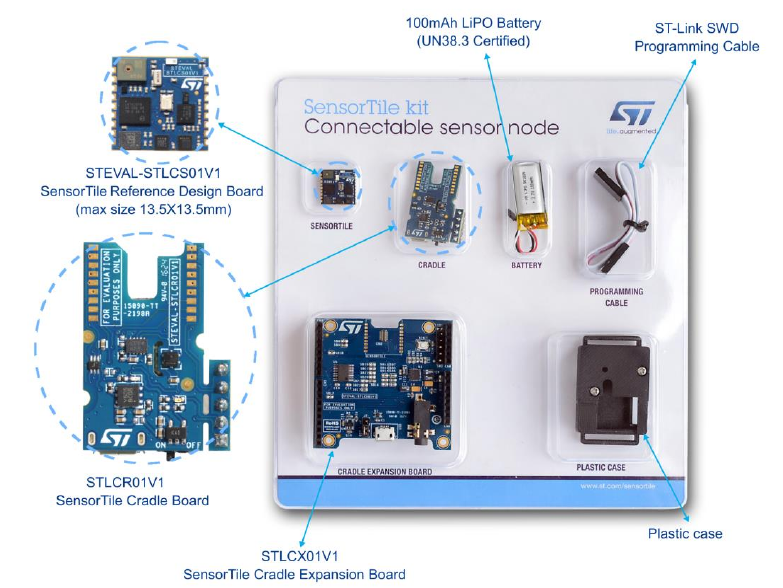
\includegraphics[scale=0.6]{sensortilekit}
\caption{SensorTile Development Kit}
\label{fig:sensortilekit}
\end{center} \end{figure}

\newpage

Figure \ref{fig:sensortile} shows position of main components of the SensorTile board, and Table \ref{table:sensortile} lists their description. \cite{stkitmanual}

\begin{figure}[H] \begin{center}
% \begin{wrapfigure}{l}{0.5\textwidth}
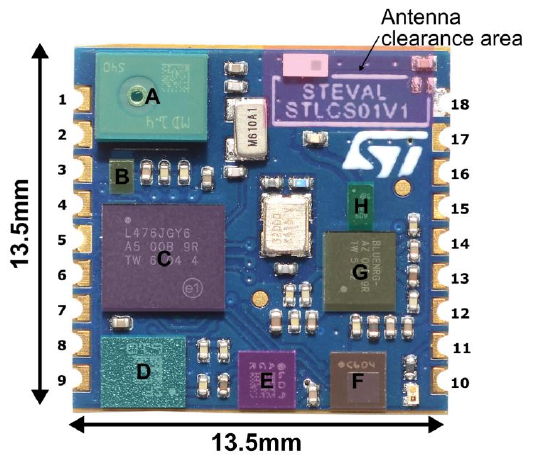
\includegraphics[scale=0.5]{sensortile}
\caption{SensorTile Main Components}
\label{fig:sensortile}
% \end{wrapfigure}
\end{center} \end{figure}

\begin{table}[H]
\centering
\begin{tabular}{@{}|c|l|p{0.55\linewidth}|@{}}
\hline
\toprule
{\bf Reference} & {\bf Device} & {\bf Description} \\ \hline
\midrule
A & MP34DT04      & MEMS audio sensor digital microphone \\ \hline
B & LD39115J18R   & 150 mA low quiescent current low noise LDO 1.8 V \\ \hline
C & STM32L476 MCU & ARM Cortex-M4 32-bit microcontroller \\ \hline
D & LSM6DSM       & iNEMO inertial module: low-power 3D accelerometer and 3D gyroscope \\ \hline
E & LSM303AGR     & Ultra-compact high-performance eCompass module: ultra-low power 3D accelerometer and 3D magnetometer \\ \hline
F & LPS22HB       & MEMS nano pressure sensor: 260-1260 hPa absolute digital output barometer \\ \hline
G & BlueNRG-MS    & Bluetooth low energy network processor \\ \hline
H & BALF-NRG01D3  & 50 Ω balun with integrated harmonic filter \\ \hline
\bottomrule
\end{tabular}
\caption{SensorTile Main Components}
\label{table:sensortile}
\end{table}

\newpage

% By default, the SensorTile comes loaded
The LSM6DSM sensor on the SensorTile board is the accelerometer and is capable of capturing data at a maximum rate of.

To interface with the sensor hardware, there are three available firmwares for the board:

\begin{enumerate}
    \item DataLogger - allows recording motion sensor data
    \item AudioLog - allows recording onboard microphone
    \item ALLMEMS - allows SensorTile to be controlled via BlueNRG android app
\end{enumerate}

Our goals with the SensorTile were two fold:

\begin{enumerate}
\item Gather data at the maximum rate possible.
\item Record both motion sensors and microphone at the same time (so that we could have a baseline to compare the sensor recordings to.)
\end{enumerate}

We didn’t succeed in achieving either of these goals as neither of the three listed stock firmwares have the capabilities that we desired. All three firmwares restricted the sensor sampling rate to around 200Hz (similar to what we would get on Android.) Another restriction was the board only allows either motion sensors OR microphone to be recorded but not both simulataneously.

Even though these firmwares are open-source, the documentation is relatively scarce, making new customizations very difficult. The SensorTile kit is relatively new, so not a lot of people are working on similar things.

\newpage
\section{Android App}

After not being able to get the SensorTile working as a better source for data, we turned back to Android and it's limited 200Hz sampling rate.

Our goals were again, to gather sensor data at the fastest rate possible and to also capture the microphone simulataneously. Since android has a plethora of apps for almost any purpose, we first tried to find an existing application that could fit our needs, but after trying out about a dozen of the apps, we found that all of them suffered from similar issues: they either didn’t have fine grained control over sampling rate for sensors Or didn’t allow both motion sensors \& microphone to be recorded at the same time.

So we designed our own application that can record Accelerometer, Gyroscope \& Microphone simultaneously at the maximum rate offered by Android. Data from the sensors is saved to separate files on disk (CSV for motion sensors and M4A for microphone.)

Figure \ref{fig:android_app_main} shows the design of our application.

\begin{figure}[H] \begin{center}
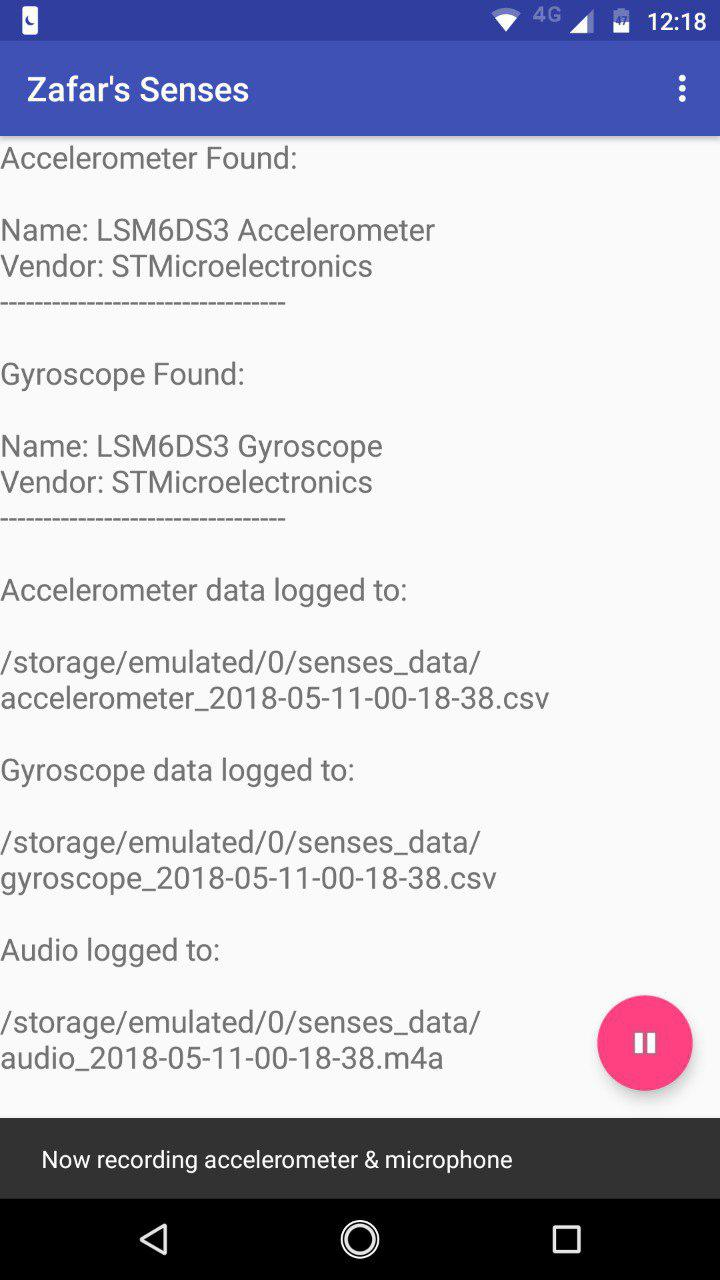
\includegraphics[scale=0.175]{android_app_main}
\caption{Sensor Data Recording App (main view)}
\label{fig:android_app_main}

% \begin{minipage}[b]{0.3\textwidth}
%   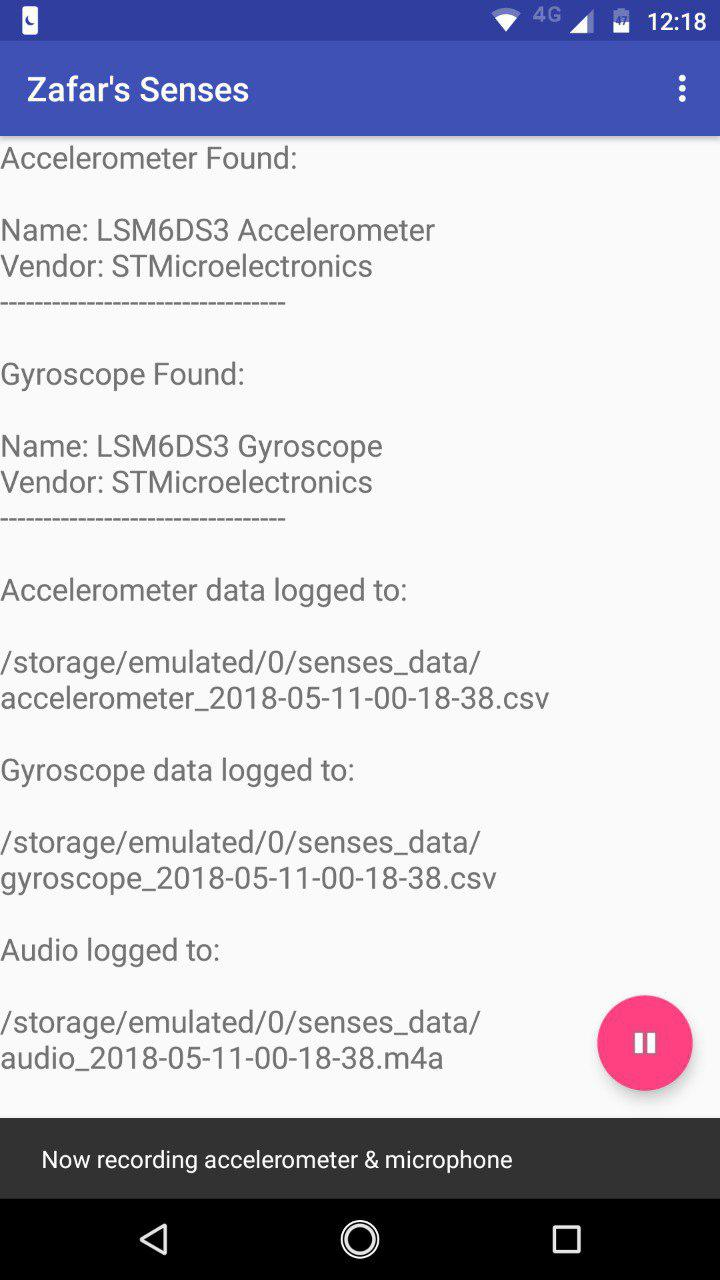
\includegraphics[width=\textwidth]{android_app_main}
%   \caption{Picture 1}
%   \label{fig:1}
% \end{minipage}

% \begin{minipage}[b]{0.3\textwidth}
%   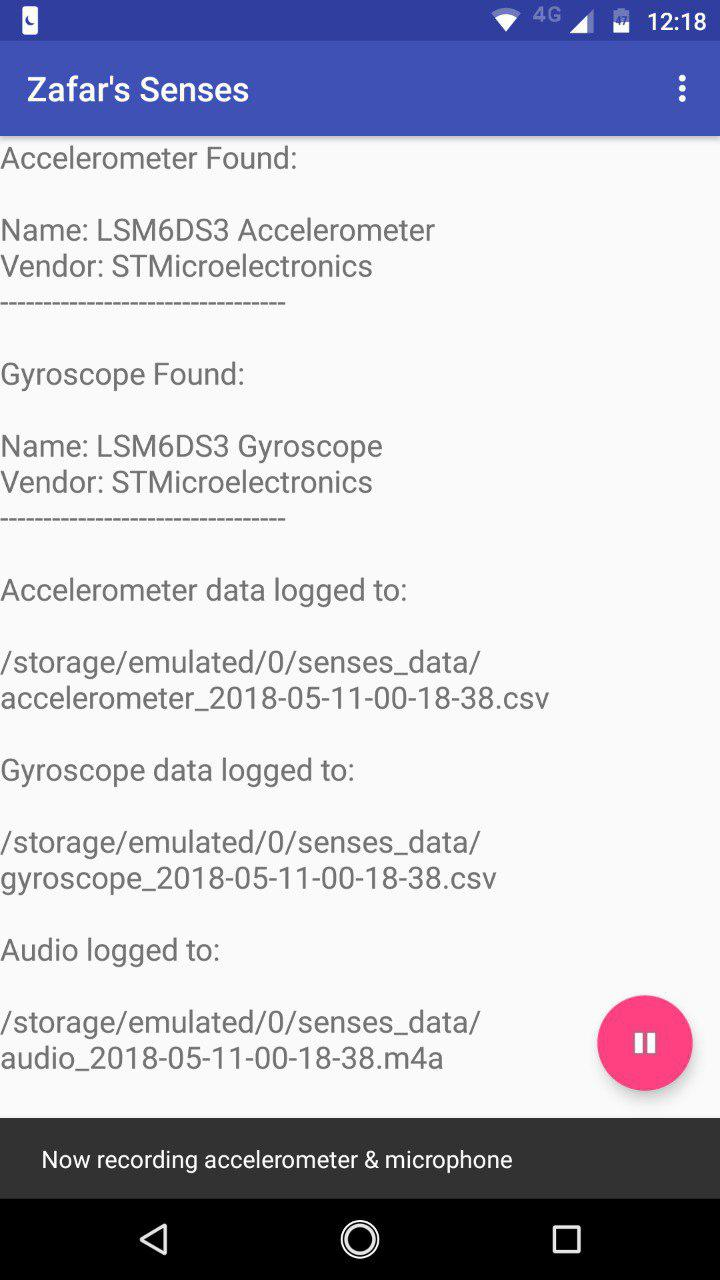
\includegraphics[width=\textwidth]{android_app_main}
%   \caption{Picture 2}
%   \label{fig:2}
% \end{minipage}

\end{center} \end{figure}

% \begin{figure}[H] \begin{center}
% 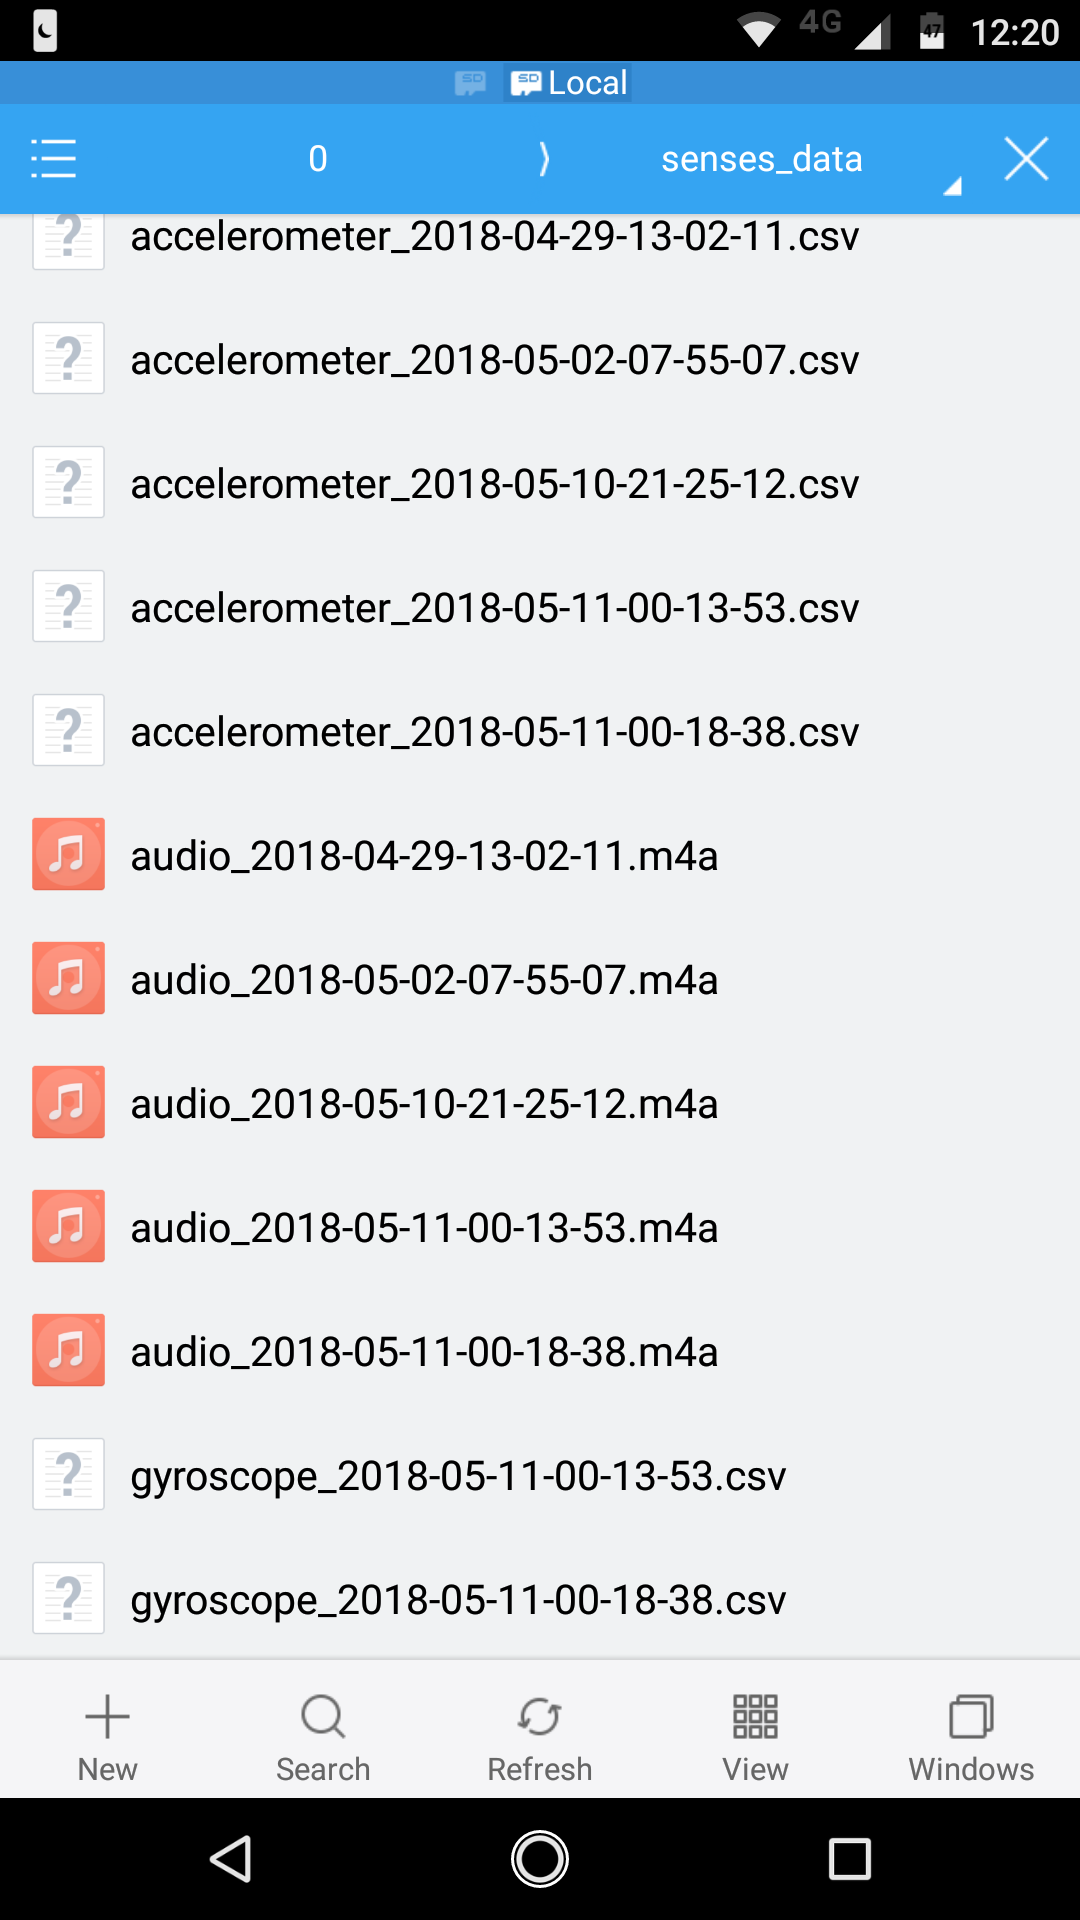
\includegraphics[scale=0.15]{android_app_files}
% \caption{Sensor Data Recording App (storage of files)}
% \label{fig:android_app_files}
% \end{center} \end{figure}

% \subfloat[Sensor Data Recording App (main view) \label{fig:1}]{%
% 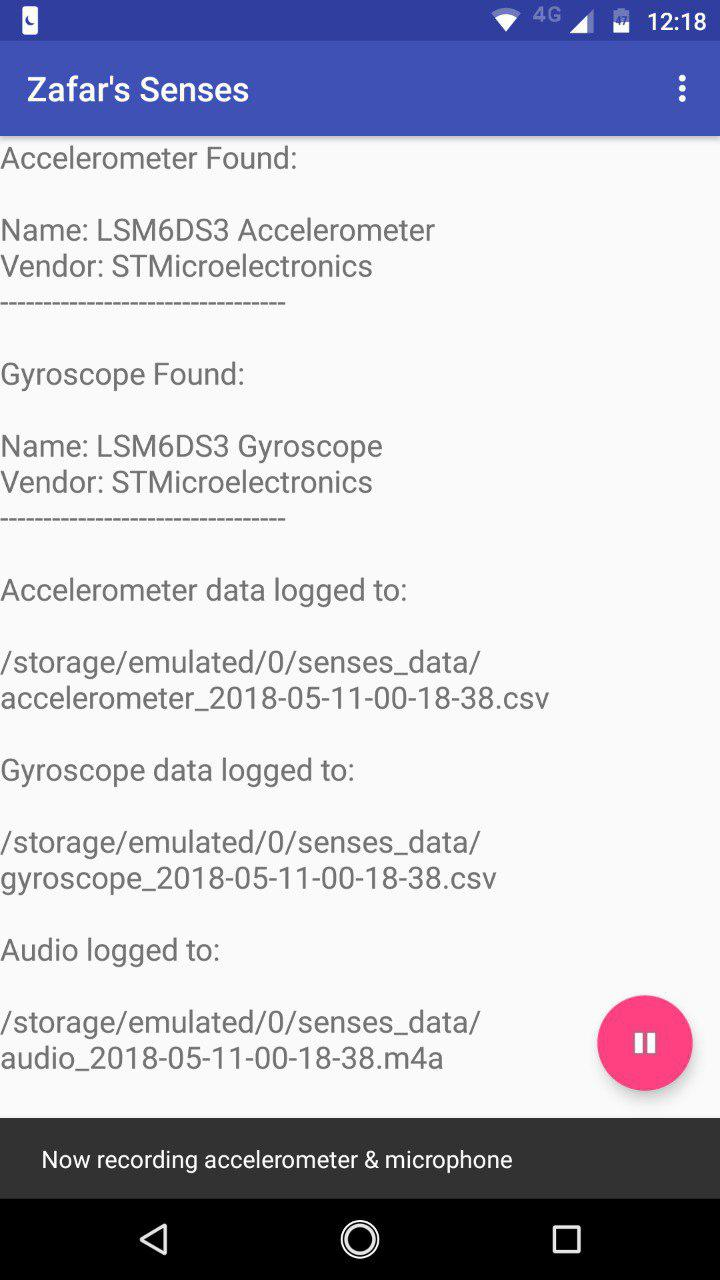
\includegraphics[width=0.5]{android_app_main.png}
% }
% \hfill
% \subfloat[Sensor Data Recording App (main view) \label{fig:2}]{%
% 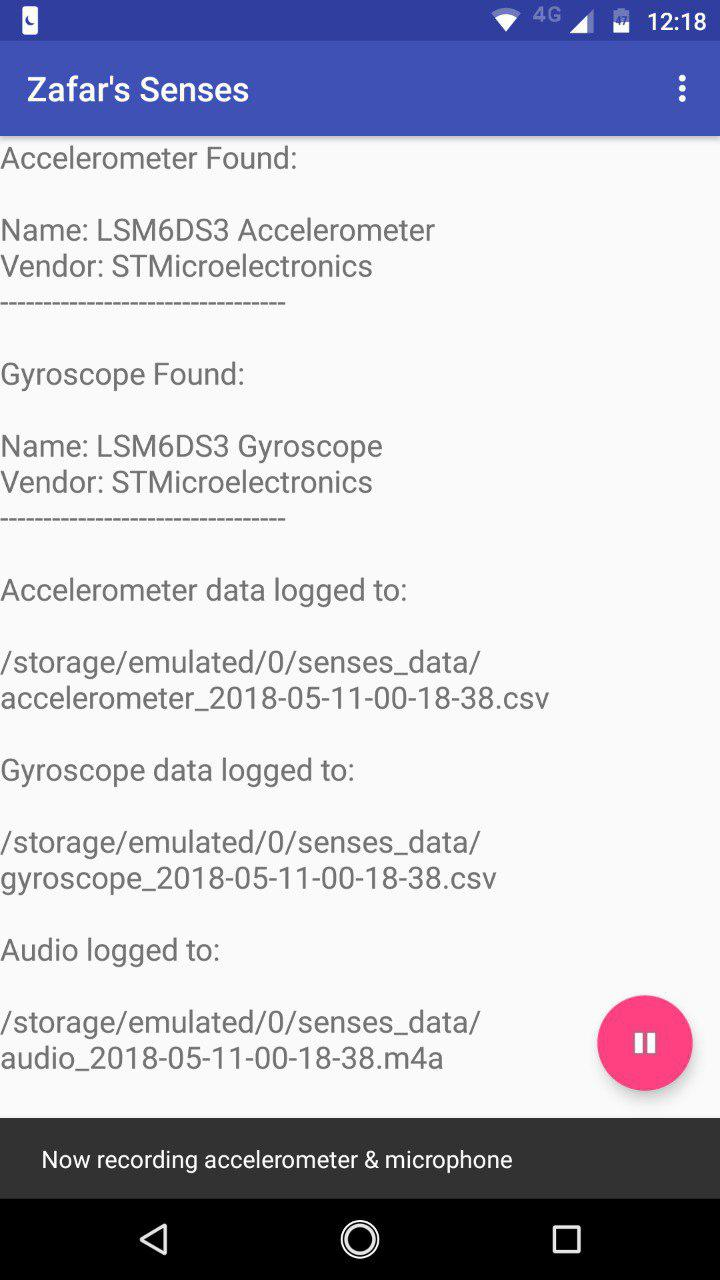
\includegraphics[width=0.5]{android_app_main.png}
% }
% \caption{Main figure caption}

